\documentclass[border=10pt]{standalone}
\usepackage[T1]{fontenc}\usepackage[utf8]{inputenc}\usepackage{lmodern}
\usepackage{tikz}\usetikzlibrary{arrows.meta,positioning,calc,fit}
\begin{document}
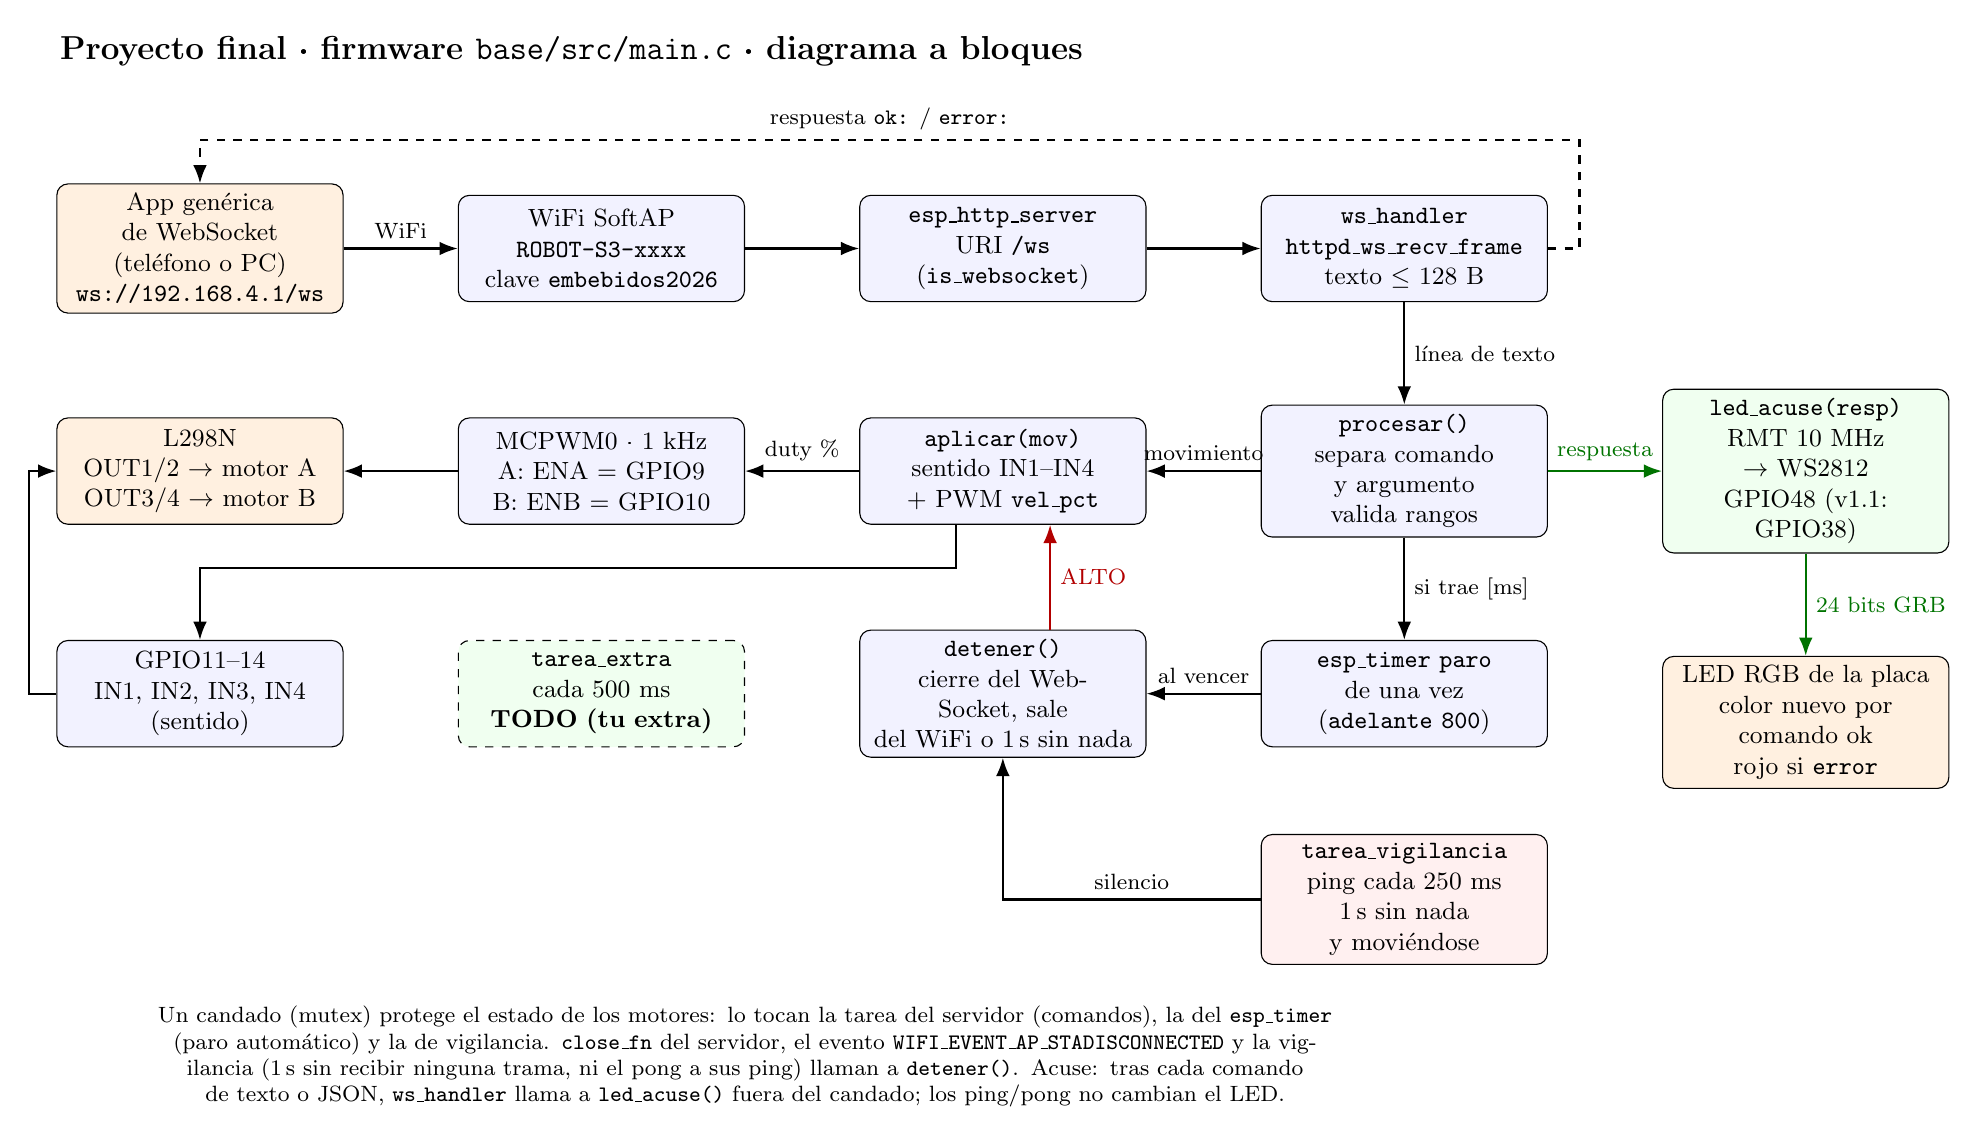
\begin{tikzpicture}[>=Latex,font=\small,node distance=0.9cm and 1.45cm,
 b/.style={draw,rounded corners,fill=blue!5,text width=3.4cm,align=center,minimum height=1.35cm},
 h/.style={draw,rounded corners,fill=orange!12,text width=3.4cm,align=center,minimum height=1.35cm},
 ex/.style={draw,rounded corners,dashed,fill=green!6,text width=3.4cm,align=center,minimum height=1.35cm}]
\node[font=\large\bfseries,anchor=west] at (-1.9,2.5) {Proyecto final · firmware \texttt{base/src/main.c} · diagrama a bloques};
% Fila 1: red
\node[h] (app) {App genérica de WebSocket\\(teléfono o PC)\\\texttt{ws://192.168.4.1/ws}};
\node[b,right=of app] (ap) {WiFi SoftAP\\\texttt{ROBOT-S3-xxxx}\\clave \texttt{embebidos2026}};
\node[b,right=of ap] (httpd) {\texttt{esp\_http\_server}\\URI \texttt{/ws}\\(\texttt{is\_websocket})};
\node[b,right=of httpd] (ws) {\texttt{ws\_handler}\\\texttt{httpd\_ws\_recv\_frame}\\texto $\le$ 128 B};
% Fila 2: logica
\node[b,below=1.3cm of ws] (proc) {\texttt{procesar()}\\separa comando y argumento\\valida rangos};
\node[b,left=of proc] (apl) {\texttt{aplicar(mov)}\\sentido IN1--IN4\\+ PWM \texttt{vel\_pct}};
\node[b,left=of apl] (pwm) {MCPWM0 · 1 kHz\\A: ENA = GPIO9\\B: ENB = GPIO10};
\node[h,left=of pwm] (l298) {L298N\\OUT1/2 $\to$ motor A\\OUT3/4 $\to$ motor B};
\node[b,fill=green!6,right=of proc] (led) {\texttt{led\_acuse(resp)}\\RMT 10 MHz $\to$ WS2812\\GPIO48 (v1.1: GPIO38)};
\node[h,below=1.3cm of led] (rgb) {LED RGB de la placa\\color nuevo por comando ok\\rojo si \texttt{error}};
% Fila 3: seguridad y extra
\node[b,below=1.3cm of proc] (timer) {\texttt{esp\_timer} \texttt{paro}\\de una vez\\(\texttt{adelante 800})};
\node[b,left=of timer] (seg) {\texttt{detener()}\\cierre del WebSocket, sale\\del WiFi o 1\,s sin nada};
\node[ex,left=of seg] (extra) {\texttt{tarea\_extra}\\cada 500 ms\\\textbf{TODO (tu extra)}};
\node[b,left=of extra] (gpio) {GPIO11--14\\IN1, IN2, IN3, IN4\\(sentido)};
\node[b,below=1.1cm of timer,fill=red!6] (vig) {\texttt{tarea\_vigilancia}\\ping cada 250 ms\\1\,s sin nada y moviéndose};
% Flechas
\draw[->,thick] (app) -- node[above,font=\footnotesize]{WiFi} (ap);
\draw[->,thick] (ap) -- (httpd);
\draw[->,thick] (httpd) -- (ws);
\draw[->,thick] (ws) -- node[right,font=\footnotesize]{línea de texto} (proc);
\draw[->,thick] (proc) -- node[above,font=\footnotesize]{movimiento} (apl);
\draw[->,thick] (apl) -- node[above,font=\footnotesize]{duty \%} (pwm);
\draw[->,thick] (pwm) -- (l298);
\draw[->,thick] ($(apl.south)+(-0.6,0)$) -- ++(0,-0.55) -| (gpio.north);
\draw[->,thick] (gpio.west) -- ++(-0.35,0) |- (l298.west);
\draw[->,thick] (proc) -- node[right,font=\footnotesize]{si trae [ms]} (timer);
\draw[->,thick,green!45!black] (proc) -- node[above,font=\footnotesize]{respuesta} (led);
\draw[->,thick,green!45!black] (led) -- node[right,font=\footnotesize]{24 bits GRB} (rgb);
\draw[->,thick] (timer) -- node[above,font=\footnotesize]{al vencer} (seg);
\draw[->,thick] (vig.west) -| node[pos=0.25,above,font=\footnotesize]{silencio} (seg.south);
\draw[->,thick,red!70!black] ($(seg.north)+(0.6,0)$) -- node[right,font=\footnotesize]{ALTO} ($(apl.south)+(0.6,0)$);
\draw[->,thick,dashed] (ws.east) -- ++(0.4,0) |- node[pos=0.75,above,font=\footnotesize]{respuesta \texttt{ok:} / \texttt{error:}} ($(app.north)+(0,0.55)$) -- (app.north);
\node[font=\footnotesize,text width=17cm,align=center,anchor=north] at ($(extra.south east |- vig.south)+(0,-0.4)$) {Un candado (mutex) protege el estado de los motores: lo tocan la tarea del servidor (comandos), la del \texttt{esp\_timer} (paro automático) y la de vigilancia. \texttt{close\_fn} del servidor, el evento \texttt{WIFI\_EVENT\_AP\_STADISCONNECTED} y la vigilancia (1\,s sin recibir ninguna trama, ni el pong a sus ping) llaman a \texttt{detener()}. Acuse: tras cada comando de texto o JSON, \texttt{ws\_handler} llama a \texttt{led\_acuse()} fuera del candado; los ping/pong no cambian el LED.};
\end{tikzpicture}
\end{document}
